\documentclass{standalone}
\usepackage{tikz}
\usetikzlibrary{patterns}
\usetikzlibrary{positioning}
\usetikzlibrary{patterns, positioning}
\usetikzlibrary{shapes.misc}
\usepackage[outline]{contour}
\contourlength{1.5pt} 
\usepackage[sfdefault]{ClearSans}

\begin{document}
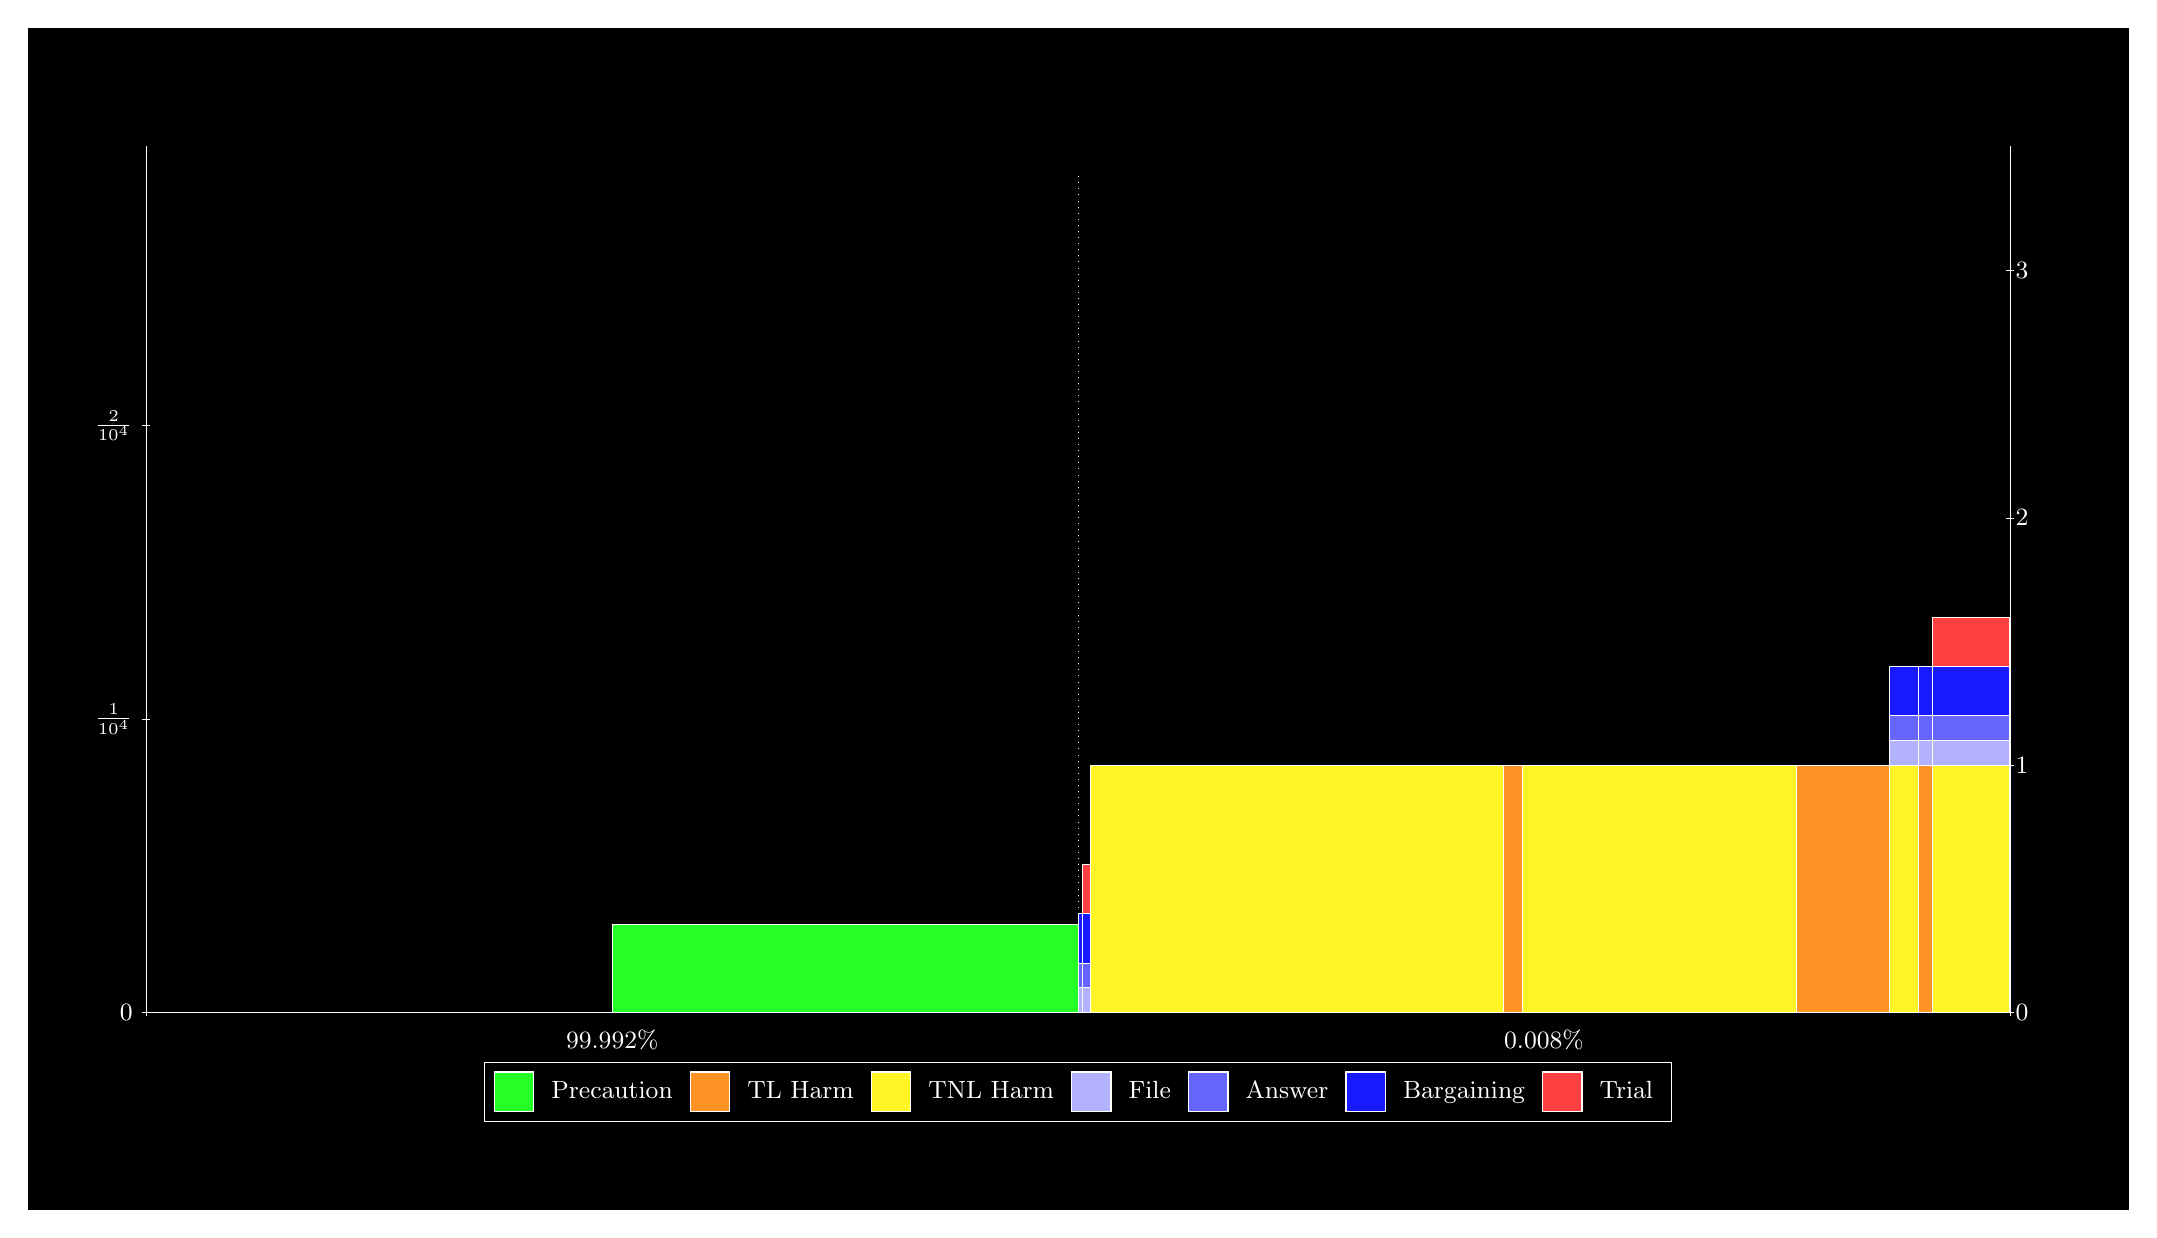
\begin{tikzpicture}
\draw[fill=black] (0,0) rectangle (26.667,15);
\draw[fill=green!85,draw=white,very thin] (7.4165,2.5) rectangle (13.333,3.6179);
\draw[fill=blue!30,draw=white,very thin] (13.333,2.5) rectangle (13.388,2.8141);
\draw[fill=blue!60,draw=white,very thin] (13.333,2.8141) rectangle (13.388,3.1281);
\draw[fill=blue!90,draw=white,very thin] (13.333,3.1281) rectangle (13.388,3.7562);
\draw[fill=blue!30,draw=white,very thin] (13.388,2.5) rectangle (13.486,2.8141);
\draw[fill=blue!60,draw=white,very thin] (13.388,2.8141) rectangle (13.486,3.1281);
\draw[fill=blue!90,draw=white,very thin] (13.388,3.1281) rectangle (13.486,3.7562);
\draw[fill=red!75,draw=white,very thin] (13.388,3.7562) rectangle (13.486,4.3844);
\draw[fill=yellow!85,draw=white,very thin] (13.486,2.5) rectangle (18.728,5.6406);
\draw[fill=orange!85,draw=white,very thin] (18.728,2.5) rectangle (18.975,5.6406);
\draw[fill=green!85,draw=white,very thin] (18.975,2.5) rectangle (22.453,2.5001);
\draw[fill=yellow!85,draw=white,very thin] (18.975,2.5001) rectangle (22.453,5.6407);
\draw[fill=green!85,draw=white,very thin] (22.453,2.5) rectangle (23.634,2.5001);
\draw[fill=orange!85,draw=white,very thin] (22.453,2.5001) rectangle (23.634,5.6407);
\draw[fill=yellow!85,draw=white,very thin] (23.634,2.5) rectangle (24.009,5.6406);
\draw[fill=blue!30,draw=white,very thin] (23.634,5.6406) rectangle (24.009,5.9547);
\draw[fill=blue!60,draw=white,very thin] (23.634,5.9547) rectangle (24.009,6.2687);
\draw[fill=blue!90,draw=white,very thin] (23.634,6.2687) rectangle (24.009,6.8969);
\draw[fill=orange!85,draw=white,very thin] (24.009,2.5) rectangle (24.177,5.6406);
\draw[fill=blue!30,draw=white,very thin] (24.009,5.6406) rectangle (24.177,5.9547);
\draw[fill=blue!60,draw=white,very thin] (24.009,5.9547) rectangle (24.177,6.2687);
\draw[fill=blue!90,draw=white,very thin] (24.009,6.2687) rectangle (24.177,6.8969);
\draw[fill=yellow!85,draw=white,very thin] (24.177,2.5) rectangle (25.156,5.6406);
\draw[fill=blue!30,draw=white,very thin] (24.177,5.6406) rectangle (25.156,5.9547);
\draw[fill=blue!60,draw=white,very thin] (24.177,5.9547) rectangle (25.156,6.2687);
\draw[fill=blue!90,draw=white,very thin] (24.177,6.2687) rectangle (25.156,6.8969);
\draw[fill=red!75,draw=white,very thin] (24.177,6.8969) rectangle (25.156,7.525);
\draw[fill=orange!85,draw=white,very thin] (25.156,2.5) rectangle (25.167,5.6406);
\draw[fill=blue!30,draw=white,very thin] (25.156,5.6406) rectangle (25.167,5.9547);
\draw[fill=blue!60,draw=white,very thin] (25.156,5.9547) rectangle (25.167,6.2687);
\draw[fill=blue!90,draw=white,very thin] (25.156,6.2687) rectangle (25.167,6.8969);
\draw[fill=red!75,draw=white,very thin] (25.156,6.8969) rectangle (25.167,7.525);
\draw[white,very thin] (1.5,2.5) -- (1.5,13.5);
\draw[white,very thin] (1.45,2.5) -- (1.55,2.5);
\node[font=\small,text=white, anchor=east] at (1.45, 2.5) {0};
\draw[white,very thin] (1.45,6.2265) -- (1.55,6.2265);
\node[font=\small,text=white, anchor=east] at (1.45, 6.2265) {$\frac{1}{10^{4}}$};
\draw[white,very thin] (1.45,9.953) -- (1.55,9.953);
\node[font=\small,text=white, anchor=east] at (1.45, 9.953) {$\frac{2}{10^{4}}$};

\draw[white,dotted,very thin] (13.333,2.83) -- (13.333,13.17);
\draw[white,very thin] (25.167,2.5) -- (25.167,13.5);
\draw[white,very thin] (25.117,2.5) -- (25.217,2.5);
\node[font=\small,text=white, anchor=west] at (25.117, 2.5) {0};
\draw[white,very thin] (25.117,5.6406) -- (25.217,5.6406);
\node[font=\small,text=white, anchor=west] at (25.117, 5.6406) {1};
\draw[white,very thin] (25.117,8.7812) -- (25.217,8.7812);
\node[font=\small,text=white, anchor=west] at (25.117, 8.7812) {2};
\draw[white,very thin] (25.117,11.922) -- (25.217,11.922);
\node[font=\small,text=white, anchor=west] at (25.117, 11.922) {3};

\draw[white,very thin] (1.5,2.5) -- (25.167,2.5);
\draw[white,very thin] (1.5,2.45) -- (1.5,2.55);
\node[font=\small,text=white, anchor=north] at (1.5, 2.45) {};
\draw[white,very thin] (25.167,2.45) -- (25.167,2.55);
\node[font=\small,text=white, anchor=north] at (25.167, 2.45) {};

\node[font=\small,text=white,anchor=south] at (7.4167, 1.9) {99.992\%};
\node[font=\small,text=white,anchor=south] at (19.25, 1.9) {0.008\%};
\draw (13.3333,2.5) node (B) {};
\begin{scope}[align=center]
\matrix[scale=0.5,draw=white,below=0.5cm of B,nodes={draw},column sep=0.1cm]{
\node[rectangle,draw,minimum width=0.5cm,minimum height=0.5cm,fill=green!85]{}; & \node[draw=none,font=\small,text=white]{Precaution}; &
\node[rectangle,draw,minimum width=0.5cm,minimum height=0.5cm,fill=orange!85]{}; & \node[draw=none,font=\small,text=white]{TL Harm}; &
\node[rectangle,draw,minimum width=0.5cm,minimum height=0.5cm,fill=yellow!85]{}; & \node[draw=none,font=\small,text=white]{TNL Harm}; &
\node[rectangle,draw,minimum width=0.5cm,minimum height=0.5cm,fill=blue!30]{}; & \node[draw=none,font=\small,text=white]{File}; &
\node[rectangle,draw,minimum width=0.5cm,minimum height=0.5cm,fill=blue!60]{}; & \node[draw=none,font=\small,text=white]{Answer}; &
\node[rectangle,draw,minimum width=0.5cm,minimum height=0.5cm,fill=blue!90]{}; & \node[draw=none,font=\small,text=white]{Bargaining}; &
\node[rectangle,draw,minimum width=0.5cm,minimum height=0.5cm,fill=red!75]{}; & \node[draw=none,font=\small,text=white]{Trial}; \\\\
};\end{scope}

\end{tikzpicture}
\end{document}